\documentclass[a4paper,12pt]{report}

\usepackage[vietnamese]{babel}
\usepackage[utf8]{inputenc, vietnam}
\usepackage[a4paper,margin=24mm]{geometry}
\usepackage[skip=10pt plus1pt, indent=20pt]{parskip}
\usepackage[colorlinks=true,allcolors=blue,urlcolor=magenta]{hyperref}

\usepackage{caption}
\usepackage{indentfirst,setspace,subcaption}
\usepackage{amsmath,amssymb,graphicx,xcolor,url}
\usepackage{fancyhdr,tocbasic,titlesec,minted,listings}

\renewcommand{\thesection}{\arabic{section}}

% Header and footer styling
\pagestyle{fancy}
\setlength{\headheight}{18pt}
\fancyhf{}
\fancyhead[R]{\nouppercase\rightmark\hfill~Báo cáo bài tập 1}
\fancyfoot[C]{\hfill\thepage\hfill}

% TOC styling
\DeclareTOCStyleEntry[
  indent=12pt,
  level=1
]{largetocline}{section}

% Title page data
\title{Báo cáo bài tập 1}
\author{\begin{tabular}{r c}
  Ngô Nguyễn Thế Khoa & 23127065
  \end{tabular}}
\date{Ngày 21 tháng 10 năm 2024}

\begin{document}

% Title page and TOC
\thispagestyle{empty}
\begin{titlepage}
	\begin{center}
		\makeatletter
		\newcommand{\HRule}{\rule{\linewidth}{0.4mm}}

		\textsc{\LARGE Vietnam National University,\\Ho Chi Minh City}\\[1.5cm]
		\textsc{\Large University of Science}\\[0.5cm]
		\textsc{\Large Faculty of Information Technology}\\[1.5cm]

		{\HRule}\\[1cm]
		{\huge \bfseries \@title}\\[0.5cm]
		{\HRule}\\[2cm]

		\textsc{\large CSC10004 -- Data Structures and Algorithms}\\[0.5cm]

		\vfill\vfill\vfill

		{\large \@author}\\[1.5cm]
		{\large \@date}
		\makeatother
	\end{center}
\end{titlepage}
\tableofcontents\thispagestyle{empty}

% Report contents
\pagebreak
\section{Đánh giá}
\subsection*{Bảng đánh giá mức độ hoàn thành}
\begin{center}
	\renewcommand{\arraystretch}{1.5}
	\begin{tabular}{|c|p{\dimexpr0.7\linewidth-\tabcolsep}|c|}
		\hline
		\textbf{STT} & \textbf{Yêu cầu}                                                                                                                                           & \textbf{Tiến độ} \\\hline
		\multicolumn{3}{|c|}{\textbf{Bài tập 1}}                                                                                                                                                     \\\hline
		1            & Nhập vào số nguyên X (4 bytes) có dấu, hãy `đọc' dãy bit nhị phân của X và xuất ra màn hình.                                                               & 100\%            \\\hline
		2            & Cho mảng 1 chiều A gồm 32 phần tử là các số 0 hoặc 1. Hãy xây dựng số nguyên X 4 bytes có các bit giống với các phần tử mảng A, sau đó xuất X ra màn hình. & 100\%            \\\hline
		\multicolumn{3}{|c|}{\textbf{Bài tập 2}}                                                                                                                                                     \\\hline
		1            & Viết chương trình nhập vào 2 dãy bit 8 bit (ở dạng bù 2)                                                                                                   & 100\%            \\\hline
		2            & Hãy thực hiện các phép tính cộng, trừ, nhân, chia trên 2 dãy bit đã nhập (Lưu ý: thực hiện theo thuật toán đã học).                                        & 100\%            \\\hline
		\multicolumn{3}{|c|}{\textbf{Tổng kết báo cáo}}                                                                                                                                              \\
		\multicolumn{3}{|c|}{\textsl{Hoàn thành 100\% yêu cầu bài tập}}                                                                                                                              \\
		\multicolumn{3}{|c|}{\textsl{Không xảy ra lỗi khi vận hành chương trình}}                                                                                                                    \\\hline
	\end{tabular}
\end{center}

\pagebreak
\section{Kết quả bài làm}
\subsection{Bài tập 1}
\begin{figure}[!ht]
	\centering
	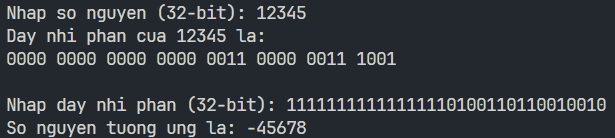
\includegraphics[width=0.9\linewidth]{imgs/1.png}
	\caption{Kết quả bài tập 1}
\end{figure}
\subsection{Bài tập 2}
\begin{figure}[!ht]
	\centering
	\begin{subfigure}{0.36\textwidth}
		\centering
		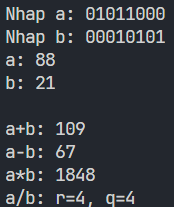
\includegraphics[width=1\textwidth]{imgs/2-1.png}
		\caption{Hình 1}
	\end{subfigure}
	\hfill
	\begin{subfigure}{0.36\textwidth}
		\centering
		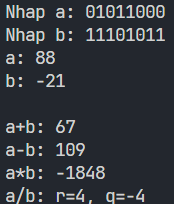
\includegraphics[width=1\textwidth]{imgs/2-2.png}
		\caption{Hình 2}
	\end{subfigure}
	\hfill
	\begin{subfigure}{0.36\textwidth}
		\centering
		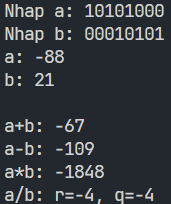
\includegraphics[width=1\textwidth]{imgs/2-3.png}
		\caption{Hình 3}
	\end{subfigure}
	\hfill
	\begin{subfigure}{0.36\textwidth}
		\centering
		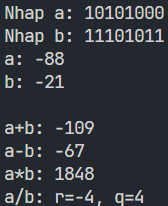
\includegraphics[width=1\textwidth]{imgs/2-4.png}
		\caption{Hình 4}
	\end{subfigure}

	\caption{Kết quả bài tập 2}
\end{figure}

\end{document}